\documentclass[openany]{report}
\usepackage[utf8]{inputenc}

\usepackage{lecture_notes_styles}
\usepackage{stylesheet}

\newtheorem{theorem}{Theorem}[section]
\newtheorem{definition}{Definition}[section]
\newtheorem{fact}{Fact}[section]
\newtheorem{prop}{Proposition}[section]
\newtheorem{corollary}{Corollary}[section]
\newtheorem{lemma}{Lemma}[section]

\title{CSI 2101 Lecture Notes}
\author{Last updated:}

\begin{document}

\maketitle

\tableofcontents
\chapter*{Definitions, Theorems, Lemmas, and Corollaries}
\label{chapter:theorems}
\addcontentsline{toc}{chapter}{\hyperref[chapter:theorems]{Definitions, Theorems, Lemmas, and Corollaries}}
\begin{manualdefinition}{\hyperref[definition4.1.1]{4.1.1}}
    Let $a$ and $b$ be two integers such that $a \neq 0$. We say that $a$ divides $b$ if there exists $c$ such that $b = ac$. If $a$ divides be we say $a$ is a factor or divisor of $b$. We also can say b is a multiple of a.

\end{manualdefinition}
\begin{manualtheorem}{\hyperref[theorem4.1.1]{4.1.1}}
    Let $a,b,c \in \ints$ with $a \neq 0$.
    \begin{enumerate}
        \item If $a\mid b$ and $a \mid c$, then $a \mid (b + c)$
        \item If $a \mid b$, then $a \mid bc$ for every integer 
        \item If $a \mid b$ and $b \mid c$, then $a \mid c$
    \end{enumerate}
\end{manualtheorem}
\begin{manualcorollary}{\hyperref[corollary4.1.1]{4.1.1}}
Let $a,b,c \in \ints$ with $a \neq 0$. If $a\mid b$ and $a \mid c$, $a \mid (mb + nc)$ for all integers $m$ and $n$
\end{manualcorollary}
\begin{manualtheorem}{\hyperref[theorem4.1.2]{4.1.2}}[The Division Algorithm]
    Let $a, d \in \ints$ with $d > 0$. There exists a unique $q$ and $r$ such that 
$$0 \leq r \leq d$$
and 
$$a = dq + r$$
We write 
$$q = a \ div \ d$$
$$r=  a \ mod \ a $$
\end{manualtheorem}

\begin{manualdefinition}{\hyperref[definition4.1.2]{4.1.2}}
        Let $a, b, m \in \ints$ with $m \geq 2$. We say $a$ is congruent to $b$ modulo $m$ if $m \mid (a-b)$. We write $a \equiv b \ (mod \ m)$
\end{manualdefinition}

\begin{manualtheorem}{\hyperref[theorem4.1.3]{4.1.3}}
        Let $a,b,c,d,m \in \ints$ with $m \geq 2$. If $a \equiv b \ (mod \ m)$ and $c \equiv d \ (mod \ m)$, then 
    \begin{enumerate}
        \item $a + c \equiv b + d \ (mod \ m)$
        \item $ac \equiv bd \ (mod \ m)$
    \end{enumerate}
\end{manualtheorem}

\begin{manualdefinition}{\hyperref[definition5.1.1]{5.1.1}}
        A positive integer $p$ is prime if it admits exactly two divisors.
\end{manualdefinition}

\begin{manualtheorem}{\hyperref[theorem5.1.1]{5.1.1}}[Fundamental Theorem of Arithmetic]
      All integers greater than 1 can be written as a product of prime numbers. This representation is unique if we write the prime numbers in non-decreasing order.
\end{manualtheorem}

\begin{manualtheorem}{\hyperref[theorem5.1.2]{5.1.2}}
     Let $n > 1$ be an integer. If $n$ is not prime, then $n$ has a prime divisor $p$ such that $p \leq \sqrt{n}$.
\end{manualtheorem}

\begin{manualcorollary}{\hyperref[corollary6.0.1]{6.0.1}}
    Let 
    $$a = p_1^{a_1} \cdot p_2^{a_2} \cdot \ldots \cdot p_k^{a_k}$$
    $$a = p_1^{b_1} \cdot p_2^{b_2} \cdot \ldots \cdot p_k^{b_k}$$
    Where $p_i$ is prime, $a_i \geq 0$ and $b_i \geq 0$, $1 \leq i \leq k$. Then 
    $$gcd(a,b) = p_1^{\min(a_1,b_1)} \cdot p_2^{\min(a_2,b_2)} \cdot \ldots \cdot p_k^{\min(a_k,b_k)}$$
    $$lcm(a,b) = p_1^{\max(a_1,b_1)} \cdot p_2^{\max(a_2,b_2)} \cdot \ldots \cdot p_k^{\max(a_k,b_k)}$$
    $$gcd(a,b) \cdot lcm(a,b) = ab$$
\end{manualcorollary}


\begin{manuallemma}{\hyperref[lemma6.0.1]{6.0.1}}
Let $a,b,q,r$ be integers such that 
    $$a = b\cdot q + r$$
    Then 
    $$gcd(a,b)=gcd(b,r)$$
\end{manuallemma}

\begin{manualdefinition}{\hyperref[definition6.0.1]{6.0.1}}[Euclidean Algorithm]
     $$x = a$$
    $$y = b$$
    while $y \neq 0$
    $$r = x \mod y$$
    $$x = y$$
    $$y = r$$
    return $x$
\end{manualdefinition}

\begin{manualtheorem}{\hyperref[theorem6.0.1]{6.0.1}}[B\'ezout]
     Let $a,b \in \ints$ be positive integers. There exists $s,t \in \ints$ such that 
    $$s \cdot a + t \cdot b = gcd(a,b)$$
\end{manualtheorem}


\begin{manuallemma}{\hyperref[lemma6.0.1]{6.0.1}}
Let $a,b,c \in \ints$ with $a \neq 0$. If $gcd(a,b) = 1$ and $a \mid (bc)$, then $a \mid c$.
\end{manuallemma}

\begin{manuallemma}{\hyperref[lemma8.0.1]{8.0.1}}
    Let $a,b,c \in \ints$, with $a \neq 0$. If $gcd(a,b) = 1$, and $a \mid (bc)$, then $a|c$.

\end{manuallemma}

\begin{manualtheorem}{\hyperref[theorem8.0.1]{8.0.1}}
        Let $a,b,c,m \in \ints$, with $m \geq 2$. Assume $ac \equiv bc \ (mod \ m)$ and $gcd(c,m) = 1$. Then $a \equiv b \ (mod \ m)$.
\end{manualtheorem}

\begin{manuallemma}{\hyperref[lemma8.0.2]{8.0.2}}
        Let $p$ be a prime number and $a_1, a_2,\dots,a_n \in \ints$.
    If $p \mid (a_1 \cdot a_2 \cdot \dots \cdot a_n)$, then there exists $1 \leq i \leq n$ such that $p \mid a_i$.
\end{manuallemma}

\begin{manualtheorem}{\hyperref[theorem8.0.2]{8.0.2}}
        Let $m \in \ints$ with $m \geq 2$ and let $a \in \ints_m$. The multiplicative inverse of $a \ (mod \ n)$ exists if and only if $gcd(a,m) = 1$. When it exists, the inverse of  $a \ (mod \ n)$ is unique.
\end{manualtheorem}

%%%%%%%%%%%%%%%%%% Lecture 1 %%%%%%%%%%%%%%%%%%%%%%%%%%%%%%%%%
\chapter{Logic and Proof Techniques}
TBC. 



%%%%%%%%%%%%%%%%%% Lecture 2 %%%%%%%%%%%%%%%%%%%%%%%%%%%%%%%%%
\chapter{Proof Examples}
TBC.

%%%%%%%%%%%%%%%%%% Lecture 3 %%%%%%%%%%%%%%%%%%%%%%%%%%%%%%%%%
\chapter{Proof by Induction and More Examples}



%%%%%%%%%%%%%%%%%% Lecture 4 %%%%%%%%%%%%%%%%%%%%%%%%%%%%%%%%%
\chapter{Intro to Number Theory}
\section{Divisibility}
\begin{definition}\label{definition4.1.1}
    Let $a$ and $b$ be two integers such that $a \neq 0$. We say that $a$ divides $b$ if there exists $c$ such that $b = ac$. If $a$ divides be we say $a$ is a factor or divisor of $b$. We also can say b is a multiple of a.
\end{definition}
\begin{theorem}\label{theorem4.1.1}
    Let $a,b,c \in \ints$ with $a \neq 0$.
    \begin{enumerate}
        \item If $a\mid b$ and $a \mid c$, then $a \mid (b + c)$
        \item If $a \mid b$, then $a \mid bc$ for every integer 
        \item If $a \mid b$ and $b \mid c$, then $a \mid c$
    \end{enumerate}
\end{theorem}
\begin{proof}
    \begin{enumerate}
        \item We have to prove if $a \mid b$ and $a\mid c$, then $a \mid (b + c)$
        Let $a,b,c \in \ints$ with $a \neq 0$. Assume that $a \mid b$ and $a \mid c$, then for some $k,l \in \ints$
        $$b = k \cdot a$$
        $$c = l \cdot a$$
        Thus, we have
        $$b + c = k \cdot a + l \cdot a  = a(k + l)$$
        So $a \mid (b+c)$
        \item We have to prove if $a \mid b$, $a \mid bc$ for every $c$. Let $a,b \in \ints$ with $a \neq 0$. Assume that $a \mid b$. Then for some $k \in \ints$,
        $$b = k \cdot a$$
        Let $c \in \ints$, so 
        $$bc = k \cdot a \cdot c = a \cdot (kc)$$
        Therefore, $a \mid bc$
        \item We have to prove if $a \mid b$ and $b \mid c$, then $a \mid c.$ Let $a,b,c \in \ints$ with $a \neq 0$. Assume $a \mid b$ and $b \mid c$. Then we have for some $k, l \in \ints$
        $$b = k \cdot a$$
        $$c = l \cdot b$$
        So, 
        $$c = l \cdot b = l \cdot (k \cdot a) = (lk)a$$
        Therefore $a \mid c$
    \end{enumerate}
\end{proof}

\begin{corollary}\label{corollary4.1.1}
Let $a,b,c \in \ints$ with $a \neq 0$. If $a\mid b$ and $a \mid c$, $a \mid (mb + nc)$ for all integers $m$ and $n$
\end{corollary}
\begin{proof}
    Let $a,b c \in \ints$ with $a \neq 0$. Assume $a \mid b$  $a \mid c$. By the previous theorem (part 2), we have $a \mid mb$ and $a \mid nc$. Therefore, by the previous theorem (part 1), $a \mid (mb + nc)$
\end{proof}
\begin{theorem}[The Division Algorithm]\label{theorem4.1.2}
Let $a, d \in \ints$ with $d > 0$. There exists a unique $q$ and $r$ such that 
$$0 \leq r \leq d$$
and 
$$a = dq + r$$
We write 
$$q = a \ div \ d$$
$$r=  a \ mod \ a $$
\end{theorem}
\begin{definition}\label{definition4.1.2}
    Let $a, b, m \in \ints$ with $m \geq 2$. We say $a$ is congruent to $b$ modulo $m$ if $m \mid (a-b)$. We write $a \equiv b \ (mod \ m)$
\end{definition}
\textbf{Example:} Prove or disprove. We have $a \equiv b \ (mod \ m)$ if and only if $b \equiv a \ (mod \ m)$
\begin{align*}
    &a \equiv b \ (mod \ m)\\
    \iff& m \mid (a - b)\tag{by definition}\\
    \iff& a - b = km\tag{$k \in \ints$}\\
    \iff& b - a = -km\\
    \iff& m \mid (b -a)\\
    \iff& b \equiv a \ (mod \ b)\tag{by definition}
\end{align*}
\begin{theorem}\label{theorem4.1.3}
    Let $a,b,c,d,m \in \ints$ with $m \geq 2$. If $a \equiv b \ (mod \ m)$ and $c \equiv d \ (mod \ m)$, then 
    \begin{enumerate}
        \item $a + c \equiv b + d \ (mod \ m)$
        \item $ac \equiv bd \ (mod \ m)$
    \end{enumerate}
\end{theorem}
    \begin{proof}
    \begin{enumerate}
        \item We have to prove $a + c \equiv b + d \ (mod \ m)$. Since $a \equiv b$ and $c \equiv d$, we have 
        $$m \mid (a - b)$$
        $$m \mid (c - c)$$
        By theorem 4.1.1 (part 1),we have 
        $$m \mid ((a-b) + (c -d)$$
        $$m \mid ((a+c) - (b + d))$$
        Therefore,
        $$a + c \equiv b + d \ (mod \ m)$$
        \item We have to prove $ac \equiv cd \ (mod \ m)$\\[1ex]
        Since $a \equiv b$ and $c \equiv d$, we have $m \mid (a-b)$ and $m \mid (c -d)$. By \hyperref[corollary4.1.1]{Corollary 4.1.1}, we have 
        $$m \mid (c(a-b)+b(c-d)$$
        $$m \mid (ac - bc + bc- bd)$$
        $$m \mid (ac - bd)$$
        Therefore $ac \equiv bd$.
    \end{enumerate}
    \end{proof}

    \section{Arithmetic Modulo m}
    Let $m \geq 2$ be an integer and 
    $$\ints_m = \{0,1,2,\dots, m-1\}$$
    We define 
    $$a +_m b = (a + b) \ (mod \ m)$$
    $$a \cdot_m b = (a \cdot b) \ (mod \ m)$$
    in $\ints_m$, this is arithmetic modulo m.
    TBC


%%%%%%%%%%%%%%%%%% Lecture 5 %%%%%%%%%%%%%%%%%%%%%%%%%%%%%%%%%
\chapter{Prime Numbers and GCD}
\section{Prime Numbers}
\begin{definition}\label{definition5.1.1}
    A positive integer $p$ is prime if it admits exactly two divisors.
\end{definition}
\begin{theorem}[Fundamental Theorem of Arithmetic]\label{theorem5.1.1}
    All integers greater than 1 can be written as a product of prime numbers. This representation is unique if we write the prime numbers in non-decreasing order.
\end{theorem}
\begin{proof}
\textbf{(Existence)} By induction,
    \begin{itemize}
        \item \textbf{Base Case:} Take $n = 2$. We have $2 = 2$, the product of 1 prime number. 
        \item \textbf{Induction Hypothesis:} Let $k \geq 2$ be an integer. Suppose that all numbers $2,3,4, \ldots, k-1, k$ can be written as a product of primes.
        \item \textbf{Induction Step:} Consider $k +1$. If $k+1$ is prime, then we're done. If not, then $K+1 = d\cdot e$ for integers $1 < d < k+1$ and $1 < e < k+1$
        By the induction hypothesis, $d$ and $e$ can be written as products of prime. So $k + 1 = d \cdot e$ can be written as a product of primes. 
    \end{itemize}
\textbf{(Uniqueness)} to be seen later.
\end{proof}
\begin{theorem}\label{theorem5.1.2}
    Let $n > 1$ be an integer. If $n$ is not prime, then $n$ has a prime divisor $p$ such that $p \leq \sqrt{n}$.
\end{theorem}
\begin{proof}
    Let $n > 1$, if $n$ is not prime, then $n = a \cdot b$ for two integers $1 < a < n$ and $1 < b < n$. We will show that $a \leq \sqrt{n}$ or $b \leq \sqrt{n}$ by contradiction. Assume $a > \sqrt{n}$ and $b > \sqrt{n}$. Then $n = a \cdot b > \sqrt{n} \cdot \sqrt{n} = n$. This is a contradiction so $a \leq \sqrt{n}$. \\[1ex] 
    Assume without loss of generality that $a \leq \sqrt{n}$. If $a$ is prime, we're done. If not, then by the fundamental theorem of arithmetic, $a$ is divisible by a prime number $p$
\end{proof}
\begin{theorem}\label{theorem5.1.3}
There exists an infinite number of prime numbers.    
\end{theorem}
\begin{proof}
    By contradiction, suppose there exists a finite number of prime numbers, say $k$ prime numbers, and we order them 
    $$p_1 < p_2 < p_3 < \cdots < p_k$$
    Consider the number 
    $$Q = p_1 \cdot p_2 \cdot \ldots \cdot p_k + 1 \in \ints$$
    Since $Q > p_k$, then $Q$ is not prime by our assumption. By \hyperref[theorem5.1.2]{Theorem 5.1.2}, Q is divisible by a prime number. So $p_i \mid Q$ for some $1 \leq i \leq k$. We also have that 
    $$p_i \mid (p_1\cdot p_2 \cdot \ldots \cdot p_i \cdot \ldots \cdot p_k)$$
    By \hyperref[corollary4.1.1]{Corollary 4.1.1}, we get
    $$p_i \mid (Q - p_1 \cdot p_2 \cdot \ldots \cdot p_k)$$
    $p_i \mid 1$
    Therefore $p_i = 1$, this is a contradiction since we assumed $p_k$ is the largest prime but $Q > p_k$ is prime. 
\end{proof}
%%%%%%%%%%%%%%%%%% Lecture 6 %%%%%%%%%%%%%%%%%%%%%%%%%%%%%%%%%
\chapter{Euclidean Algoirthm and B\'ezout's Theorem}
\begin{corollary}\label{corollary6.0.1}
    Let 
    $$a = p_1^{a_1} \cdot p_2^{a_2} \cdot \ldots \cdot p_k^{a_k}$$
    $$a = p_1^{b_1} \cdot p_2^{b_2} \cdot \ldots \cdot p_k^{b_k}$$
    Where $p_i$ is prime, $a_i \geq 0$ and $b_i \geq 0$, $1 \leq i \leq k$. Then 
    $$gcd(a,b) = p_1^{\min(a_1,b_1)} \cdot p_2^{\min(a_2,b_2)} \cdot \ldots \cdot p_k^{\min(a_k,b_k)}$$
    $$lcm(a,b) = p_1^{\max(a_1,b_1)} \cdot p_2^{\max(a_2,b_2)} \cdot \ldots \cdot p_k^{\max(a_k,b_k)}$$
    $$gcd(a,b) \cdot lcm(a,b) = ab$$
\end{corollary}
\textbf{Example:} 
\begin{align*}
    24 &= 2^3 \cdot 3\\
    36 &= 2^2 \cdot 3^2\\
    gcd(24,36) &= 2^2 \cdot 3^1 = 12\\
    lcm(24,36) &= 2^3 \cdot 3^2 = 72\\
    12 \cdot 72 &= 864 = 24 \cdot 36
\end{align*}
\begin{lemma}\label{lemma6.0.1}
    Let $a,b,q,r$ be integers such that 
    $$a = b\cdot q + r$$
    Then 
    $$gcd(a,b)=gcd(b,r)$$
\end{lemma}
\begin{proof}
     Let $a,b,q,r$ be integers such that 
     $$a = bq + r$$
     Let $d \in \ints$. We will prove that 
    $$d \mid a \wedge d \mid b \iff d \mid b \wedge d\mid r$$
    ($\implies$) Let $d \in \ints$. Assume $d \mid a$ and $d \mid b$. Then $d \mid (1 \cdot a + (-q)\cdot b)$, by \hyperref[corollary4.1.1]{Corollary 4.1.1}. Then $a = bq + r \implies r = a -bq$, so $d \mid (1 \cdot a + (-q)\cdot b) \implies d \mid r$.\\[2ex]
    ($\impliedby$) Let $d \in \ints$. Assume $d \mid b$ and $d \mid r$. Then $d \mid (q\cdot b + 1 \cdot r)$ by \hyperref[corollary4.1.1]{Corollary 4.1.1}. Then $d \mid a$, therefore $d \mid a$ and $d \mid b$
\end{proof}
\textbf{Example:} $gcd(414,662)$, $662 = 1 \cdot 414 + 248$
\begin{align*}
    662 &= 1 \cdot 414 + 248\\
    414 &= 1 \cdot 248 + 166\\
    248 &= 1 \cdot 166 + 82\\
    166 &= 2 \cdot 82 + 2 \\
    82 &= 41 \cdot 2 + 0
\end{align*}
The last none-zero remainder of this sequence is the $gcd$ of 414 and 662 by the previous lemma. (can someone find which lemma this is!)
\begin{definition}[Euclidean Algorithm]\label{definition6.0.1}
    $$x = a$$
    $$y = b$$
    while $y \neq 0$
    $$r = x \mod y$$
    $$x = y$$
    $$y = r$$
    return $x$
\end{definition}
This algorithm returns the $gcd$ of $a$ and $b$.\\[3ex]
\textbf{Example:}$gcd(465,144)$
\begin{align*}
    465 &= 3 \cdot 144 + 33\\
    144 &= 4 \cdot 33 + 12\\
    33 &= 2 \cdot 12  + 9\\
    12 &= 1 \cdot 9 + 3 \\
    9 &= 3 \cdot 3 + 0
\end{align*}
Therefore $gcd(465,144) = 3$. 
\begin{center}
    \red{\textbf{Note: When you show the trace of Euclid's algorithm, you must include the last line with a remainder of 0.}}
\end{center}
\begin{theorem}[B\'ezout]\label{theorem6.0.1}
    Let $a,b \in \ints$ be positive integers. There exists $s,t \in \ints$ such that 
    $$s \cdot a + t \cdot b = gcd(a,b)$$
\end{theorem}
\begin{proof}
    Let $a,b \in \nat \setminus \{0\}$. Run Euclidian algorithm, and assume without loss of generality $b \leq a$.
    \begin{align*}
        a &= q \cdot b + r\\
        r_0 &= q_1 \cdot r_1 + r_2\\
        r_1 &= q_2 \cdot r^2 + r_3\\
        r_2 &= q_3 \cdot r_3 + r_4\\
        \vdots \\
        r_{n-3} &= q_{n-2} \cdot r_{n-2} + r_{n-1}\\
        r_{n-2} &= q_{n-1} \cdot r_{n-1} + r_{n}\\
        r_{n-1} &= q_{n} \cdot r_{n} + 0\\
    \end{align*}
    Then, we have 
    \begin{align*}
        gcd(a,b) &= r_n\\
        &= r_{n-2} - q_{n-1} \cdot r_{n-1}\\
        &= r_{n-2} - q_{n-1}(r_{n-3} - q_{n-2}r_{n-2})\\
        &= r_{n-2} - q_{n-1}(r_{n-3} - q_{n-2}r_{n-2})\\
        &= - q_{n-1}\cdot + (1 + q_{n-2}q_{n-1})\cdot r_{n-2}\\
        \vdots \\
        &= s \cdot r_0 + t \cdot r_1\\
        &= s \cdot a + t \cdot tb
    \end{align*}
    So we read the trace of Euclid's algorithm backward while keeping $gcd(a,b)$ on the same side of the equality.
\end{proof}
\textbf{TBC.}
\begin{lemma}\label{lemma6.0.2}
    Let $a,b,c \in \ints$ with $a \neq 0$. If $gcd(a,b) = 1$ and $a \mid (bc)$, then $a \mid c$.
\end{lemma}
\begin{proof}
    Assume $gcd(a,b) = 1$ and $a \mid (bc)$. By B\'ezout, there exist $s,t \in \ints$ such that 
    \begin{align*}
        s \cdot a + t \cdot b &= gcd(a,b) = 1\\
        s \cdot a \cdot c + t \cdot b \cdot c &= c\tag{*}
    \end{align*}
    Since $a \mid a$ and $a \mid (bc)$, we have 
    $$a \mid (s \cdot c \cdot a + t \cdot b \cdot c$$
    By \hyperref[corollary4.1.1]{Corollary 4.1.1}. Then from (*), this means 
    $$a \mid c$$
\end{proof}
%%%%%%%%%%%%%%%%%% Lecture 7 %%%%%%%%%%%%%%%%%%%%%%%%%%%%%%%%%
\chapter{Applications of B\'ezout's Theorem}
TBC. 

\chapter{GCD and Modulo n, Multiplicative Inverses in Modulo n}
\begin{lemma}\label{lemma8.0.1}
Let $a,b,c \in \ints$, with $a \neq 0$. If $gcd(a,b) = 1$, and $a \mid (bc)$, then $a|c$.
\end{lemma}
\begin{proof}
    Seen last week.
\end{proof}
\begin{theorem}\label{theorem8.0.1}
    Let $a,b,c,m \in \ints$, with $m \geq 2$. Assume $ac \equiv bc \ (mod \ m)$ and $gcd(c,m) = 1$. Then $a \equiv b \ (mod \ m)$.
\end{theorem}
\begin{proof}
    Let $a,b,c,m \in \ints$ with $m \geq 2$. Assume $ac \equiv bc \ (mod \ m)$ and $gcd(c,m) = 1$.
    \begin{align*}
        m \mid (ac-bc)\tag{def of mod}\\
        m \mid (c(a-b))\\
        m \mid (a-b)\tag{by previous lemma}\\
        a \equiv b \ (mod \ m)\tag{def of mod}
    \end{align*}
\end{proof}
\begin{lemma}\label{lemma8.0.2}
    Let $p$ be a prime number and $a_1, a_2,\dots,a_n \in \ints$.
    If $p \mid (a_1 \cdot a_2 \cdot \dots \cdot a_n)$, then there exists $1 \leq i \leq n$ such that $p \mid a_i$.
\end{lemma}
\begin{proof}
    By induction on $n$.
    \begin{itemize}
        \item \textbf{Base Case:} $n = 1$. Let $p$ be a prime number, if $p \mid a_1$, then $p\mid a_1$
        \item \textbf{Induction Hypothesis:} Let $k \geq 1$ be an integer. Suppose that for all integers $a_1, a_2, \dots, a_k$
        $$p\mid(a_1 \cdot a_2 \cdot \ldots \cdot a_k) \implies \exists 1 \leq i \leq k \ s.t \ p\mid a_i$$
        If $p \mid a_{k+1}$, then we're done. If not, then 
        $$gcd(p,a_{k+1}) = 1$$
        So $p\mid(a_1 \cdot a_2 \cdot \ldots \cdot a_k)$ by the previous lemma. By the induction hypthesis, ther exists $1 \leq i \leq k$ such that $p \mid a_i$.
    \end{itemize}
    \item \textbf{Induction Step:} Suppose
    $$p \mid (a_1 \cdot a_2 \cdot \ldots \cdot a_k \cdot a_{k+1})$$
\end{proof}
\begin{theorem}\label{theorem8.0.2}
    Let $m \in \ints$ with $m \geq 2$ and let $a \in \ints_m$. The multiplicative inverse of $a \ (mod \ n)$ exists if and only if $gcd(a,m) = 1$. When it exists, the inverse of  $a \ (mod \ n)$ is unique.
\end{theorem}
\begin{proof}
    Let $m\in \ints$ with $m \geq 2$ and $a \in \ints_m$\\[2ex]
    \textbf{($\implies$):} Assume the multiplicative inverse of  $a \ (mod \ n)$ exists. Let $\bar{a}$ be this inverse. By definition,
    \begin{align*}
        a \cdot \bar{a} &\equiv 1 \ (mod \ m)\\
        m &\mid (a \cdot \bar{a} - 1)\tag{def. of modulo}
    \end{align*}
    Then, $a \cdot \bar{a} - 1 = k \cdot m$ for some $m \in \ints$. Let $d = gcd(a,m)$ Then $d|a$ and $d|m$. By a result seen in class, 
    \begin{align*}
        d &\mid (\bar{a} \cdot a + (-k)m)\\
        d &\mid 1
    \end{align*}
    So, $d = 1$\\[2ex]
    \textbf{($\impliedby$):} Assume $gcd(a,m) = 1$. By B\'ezout, there exists $s,t \in \ints$ such that 
    $$s\cdot a + t \cdot m = gcd(a,m) = 1$$
    \begin{align*}
        s \cdot a + t \cdot m \equiv 1 \ (mod \ m)\\
        s \cdot a + t \cdot 0 \equiv 1\ (mod \ m)\\
        s \cdot a \equiv 1 \ (mod \ m)\\
    \end{align*}
    So, we can take $\bar{a} \equiv s \ (mod \ m)$\\[2ex]
    \textbf{(Uniqueness):} Consider two arbitrary multiplicative inverses of $a \ (mod \ m)$. Denote them by, $s, s' \in \ints_m$. So by definition
    $$sa \equiv 1 \ (mod \ m) \text{ and } s'a \equiv 1 \ (mod \ m)$$
    Then $gcd(a,m) = 1$ by the previous proof, also we have 
    \begin{align*}
        sa &\equiv s'a \ (mod \ m)\\
        m &\mid (sa - s'a)\tag{def. of modulo}\\
        m &\mid (a(s-s'))\\
        m &\mid (s-s')\tag{since $gcd(a,m)=1$}\\
        s &\equiv s' \ (mod \ m)\tag{def. of modulo}
    \end{align*}
    Therefore, $s$ and $s'$ are the same in $\ints_m$.
\end{proof}
\textbf{Example:} Find the multiplicative inverse of 101 (mod 4620).\\[2ex]
\textbf{Euclid:}
\begin{align*}
    4620 & = 45 \cdot 101 + 75\\
    101 &= 1 \cdot 75 + 26\\
    75 &= 2 \cdot 26 + 23\\
    26 &= 1 \cdot 23 + 3\\
    23 &= 7 \cdot 3 + 2\\
    3 &= 1 \cdot 2 + 1\\
    2 &= 2\cdot1 + 0
\end{align*}
\textbf{B\'ezout:}
\begin{align*}
    1 &= 3 - 1\cdot 2\\
    1 & = 3 - 1 \cdot (23 -  7 \cdot 3)\\
    1 & = 3 - 1\cdot 23 + 7\cdot 3\\
    1 &= 8\cdot 3  - 1\cdot 23\\
    1 &= -1 \cdot 23 + 8 \cdot 3\\
    1 &= -1 \cdot 23 + 8 \cdot (26 - 1 \cdot 23)\\
    1 &= -1 \cdot 23 + 8 \cdot 26 - 8 \cdot 23\\
    1 &= -9 \cdot 23 + 8\cdot 26\\
    1 &= 8 \cdot 26 - 9 \cdot 23\\
    1 &= 8 \cdot 26 - 9 \cdot (75 - 2 \cdot 26)\\
    1 & = 8 \cdot 26 - 9\cdot 75 + 18 \cdot 26\\
    1 &= -9 \cdot 75 + 26 \cdot 26\\
    1 &= -9 \cdot 75 + 26 \cdot (101 - 1 \cdot 75)\\
    1 &= -9 \cdot 75 + 26 \cdot 101 -26 \cdot 75\\
    1 &= 26 \cdot 101 - 35 \cdot 75\\
    1 &= 26 \cdot 101 - 35 \cdot (4620 - 45\cdot 101)\\
    1 &= 26\cdot 101 - 35 \cdot 4620 + 1575\cdot 21\\
    1 &= -35 \cdot 4620 + 1601 \cdot 101
\end{align*}
So,
\begin{align*}
    -35 \cdot 4620 + 1601 \cdot 101 &\equiv 1 \ (mod \ 4620)\\
    -35 \cdot 0 + 1601 \cdot 101 &\equiv 1 \ (mod \ 4620)\\
    1601 \cdot 101 &\equiv 1 \ (mod \ 4620)\\
    101 &\equiv 1601 \ (mod \ 4620)
\end{align*}
Therefore, the inverse of 101 in $\ints_{4620}$  is 1601. \\[3ex]
\textbf{Example:} Find the multiplicative inverses in $\ints_{10}$.
\begin{itemize}
    \item $\bar{0}$ does not exist since $gcd(0,10) = 10 \neq 1$
    \item $\bar{1} \equiv 1 \ (mod \ 10)$
    \item $\bar{2}$ does not exist since $gcd(2,10) = 2 \neq 1$
    \item $\bar{3} \equiv 7 \ (mod \ 10)$
    \item $\bar{4}$ does not exist since $gcd(4,10) = 2 \neq 1$
    \item $\bar{5}$ does not exist since $gcd(5,10) = 5 \neq 1$
    \item $\bar{6}$ does not exist since $gcd(6,10) = 2 \neq 1$
    \item $\bar{7} \equiv 3 \ (mod \ 10)$
    \item $\bar{8}$ does not exist since $gcd(8,10) = 2 \neq 1$
    \item $\bar{9} \equiv 9 \ (mod \ 10)$
\end{itemize}
\begin{center}
    \textbf{This concludes the material for midterm 1.}
\end{center}
\chapter{Solving Congruences}
\begin{definition}[Linear Congruence]
$ax \equiv b$ (mod $m$)
\end{definition}
\textbf{Example:}
$$3x \equiv 5 \ (mod \ 7)$$
$$x \equiv 0 \ (mod \ 7)$$
$$x - 0 = 7k$$
\textbf{Question:} What is the multiplicative inverse of $3$ (mod $7$)
So we have $3x \equiv 5$ (mod $7$). 
$$15x \equiv 25 \ (mod \ 7)$$
$$x \equiv 4 \ (mod \ 7)$$
$$3 \cdot 4 = 12 \equiv 5 \ (mod \ 7)$$

\section{Linear Congruence System}
Find $x$ such that
$$x \equiv a_1 \ (mod \ m_1)$$
$$x \equiv a_2 \ (mod \ m_n)$$
$$\vdots$$
$$x \equiv a_n \ (mod \ m_n)$$

\textbf{Example:}
$$x \equiv 2\ (mod \ 3)$$
$$x \equiv 3\ (mod \ 5)$$
$$x \equiv 5\ (mod \ 7)$$
Try $x = 68$
$$68 \equiv 2 \ (mod \ 3)$$
$$68 \equiv 3 \ (mod \ 5)$$
$$68 \equiv 5 \ (mod \ 7)$$
So, $x = 68$ is a solution to the system.
\subsection{Substitution Method}
$$x \equiv 2 \ (mod \ 3)$$
$$x = 3 \cdot t + 2$$
For some $t \in \ints$
$$x \equiv \ (mod \ 5)$$
$$3t + 2 \equiv 3 \ (mod \ 5)$$
$$3t \equiv 1 \ (mod \ 5)$$
Multiply $3x$ by the multiplicative inverse of $3$ in $\ints_5$.
$$2 \cdot 3t \equiv 2 \cdot 1 \ (mod \ 5)$$
$$t \equiv 2 \ (mod \ 5)$$
$$t = 5u + 2 \ (mod \ 5)$$ 
For an $u \in \ints$\\
\begin{center}
    \[\begin{rcases}
$$x = 3t + 2$$\\
$$t = 5u + 2$$
\end{rcases}\] $\implies x =$ ?
\end{center}
$$x = 3(5u +2) +2 = 15u + 8$$

\begin{align*}
15u + 8 &\equiv 5 \ (mod \ 7)\\
15u &\equiv -3 \ (mod \ 7)\\ 
15u &\equiv 4 \ (mod \ 7) \\
15u - 14u &\equiv 4 \ (mod \ 7)\\
u &\equiv 4 \ (mod \ 7)
\end{align*}
So $u = 7v + 4$ for some $v \in \ints$. Thus,
\begin{align*}
    x &= 15u + 8\\
    &= 15(7v + 4) + 8\\
    &= 105v + 68
\end{align*}
So,
\begin{align*}
    105v + 68 &\equiv 2 \ (mod \ 3)\\
    105v + 68 &\equiv 3\ (mod \ 5)\\
    105v + 68 &\equiv 5\ (mod \ 7)\\
\end{align*}

\noindent
\textbf{Example:}
\begin{align*}
    x &\equiv 1 \ (mod \ 4)\\
    x &\equiv 3 \ (mod \ 5)
\end{align*}
Then $x = 4t + 1$ for some $t \in \ints$. Then from the second equation, we get 
\begin{align*}
    4t + 1 &\equiv 3 \ (mod \ 5)\\
    4t + 1 - 1 &\equiv 3 -1 \ (mod \ 5)\\
    4t  &\equiv 2 \ (mod \ 5)\\
    4\cdot4t  &\equiv 4\cdot2 \ (mod \ 5)\\
    16t  &\equiv 8 \ (mod \ 5)\\
    16t  &\equiv 8 \ (mod \ 5)\\
    16t - 15t  &\equiv 8 - 5\ (mod \ 5)\\
    t  &\equiv 3\ (mod \ 5)\\
\end{align*}
Thus, $t = 5u + 3$ for some $u \in \ints$. So $x = 20u + 13$ is a solution to the system. 
\begin{align*}
    20u + 13 &\equiv 1 \ (mod \ 4)\\
    20u + 13 &\equiv 3 \ (mod \ 5)\\
\end{align*}

\noindent
\textbf{Question:} Are there systems that admit no solution? Consider
$$x \equiv 2 \ (mod \ 4)$$
$$x \equiv 3 \ (mod \ 6)$$
So $x = 4t + 2$ for some $t \in \ints$
$$4t + 2 \equiv 3 \ (mod \ 6)$$
$$4t \equiv 1 \ (mod \ 6)$$
But, 4 does not have a multiplicative inverse in $\ints_6$ since $gcd(4,6)\neq 1$. 
\begin{theorem}[Chinese Remainder Theorem]
Let $m_1, m_2, \dots, m_r \in \ints$ be pairwise co-prime integers such that $m_i \geq 2$ for $1 \leq i \leq r$
\end{theorem}
\begin{definition}[Pairwise Co-prime]
    $gcd(m_i,m_j) = 1$
\end{definition}
Let $a_1, a_2, \dots, a_r \in \ints$, then the system
\begin{align*}
    x &\equiv a_1 \ (mod \ m_1)\\
    x &\equiv a_2 \ (mod \ m_2)\\
    &\vdots\\
    x &\equiv a_r \ (mod \ m_r)
\end{align*}
admits a unique solution $(mod \ m_1 \cdot m_2 \cdots m_r)$.In other words, the solution exists and is unique in $\ints_{m_1 \cdot m_2 \cdots m_r}$\\[2ex]
Consider the system
\begin{align*}
    x \equiv 2 \ (mod \ 3)\\
    x \equiv 3 \ (mod \ 5)\\
    x \equiv 5 \ (mod \ 7)\\
\end{align*}
So we have $\ints_{3 \cdot 5 \cdot 7} = \ints_{105}$, $68 \in \ints_{105}$ and $x = 105u + 68$. 

\chapter{Fermat's Theorem}
\begin{theorem}[Fermat's Theorem]
    Let $p,a \in \ints$ such that $p$ is prime, then 
    \begin{enumerate}
        \item
    $$a^p \equiv a \ (mod \ p)$$
        \item
    If $gcd(a,p) = 1$, then $a^{p-1} \equiv 1 \ (mod \ p)$
        
    \end{enumerate}
\end{theorem}
\noindent
\textbf{Example:} 
$$1534^{2016} \pmod{2017}$$
2017 is prime and $1534 < 2017$, so $gcd(1534, 2017) = 1$ and $1534^{2016} \equiv 1 \ (\mod \ 2017)$
\begin{proof}For (2), we need to usthe following property
\[1 \cdot a, 2\cdot a, 3 \cdot a, \dots, (p-1)\cdot a\] 
are all different$\pmod{p}$.Consider $s, e \in \{1, 2, \ldots, p-1\}$ such that 
\[ra \equiv sa \pmod{p}\]
Since $\gcd(a,p) = 1$, we can divide both sides by $a$ to get 
\[r \equiv s \pmod{p}\]
Then since $r, s < p$, then $r = s$`'

\end{proof}

%------------ Skip Lecture 11 ------------
\setcounter{chapter}{11}

%----------------- Lecture 12 -----------------
\chapter{Intro to Cryptography}

%----------------- Lecture 13 -----------------
\chapter{Asympotic Notation}

\section{Big-O Notation}
The \emph{O-notation} describes an asympotic upper bound.
\begin{definition}
    Let 
    \[f: \nat \rightarrow \real^+\]
    \[g: \nat \rightarrow \real^+\]
    be two functions. We say that $f$ is \emph{O(g)} if there exists a real number $c > 0$ and $k \in \nat$ such that for all $n \geq k$, 
    \[f(n) \leq c \cdot g(n)\]
\end{definition} 
\noindent
\textbf{Notation:}
\[f(n) \leq c \cdot g(n)\]
\[f = O(g)\]
\[\exists c\exists k \forall n (n \geq k \implies f(n) \leq c \cdot g(n))\]
\textbf{Domain:} $k, n \in \nat$, $c \in \real^+ \setminus \{0\}$\\[3ex]
\noindent
\textbf{Example:} $13x^3 + 12x^2 + 5 = O(x^3)$. We have
\[13x^3 + 12x^2 + 5 \leq 13x^3 + 12x^3 + 5x^2 = 30x^3\]
Take $c = 30$ and $k = 1$. So 
\[13x^3 + 12x^2 + 5 \leq 30 \cdot x^3 \]
for all $x \geq 1$. Therefore $13x^3 + 12x^2 + 5 = O(x^3)$. \\[3ex]
\textbf{Example:} $x^2 = O\left(\frac{1}{2}x^2 - 10x\right)$. We have 
\[x^2 \leq 2 \left(\frac{1}{2}x^2 - 10x\right)\]
Now we want 
\[x^2 \geq 40x\]
so that that $x^2 - 40x$ is positive. So
\[x > 40\]
Then, 
\begin{align*}
    x^2 &= 2x^2 - x^2\\
    &\leq 2x^2 - 40x\\
    &= 4\left(\frac{1}{2}x^2 - 10x\right)
\end{align*}
So take $c = 4$ and $k = 40$. Then $x^2 = O\left(\frac{1}{2}x^2 - 10x\right)$ for all $x \geq 40$.


\begin{prop}
    Let $a > 0$ and $b > 0$. be two rael numbers. We have 
    \[log^a(x) = O(x^b)\]
\end{prop}
\begin{proof}
    Let $a > 0$ and $b > 0$ be two real numbers. We'll use that fact that $\forall x \geq 0$, we have $x \leq e^x$. From which, we have $log(x) \leq x$. Let $x$ be an integer. We have, by the previous property, 
    \begin{align*}
        \log(x^{\frac{b}{a}}) &\leq x^{\frac{b}{a}}\\
        \frac{b}{a}\log(x) &\leq x^{\frac{b}{a}}\\
        \left(\frac{b}{a}\right)^a \log^a(x) &\leq x^b\\
        \log^a(x) &\leq \left(\frac{a}{b}\right)^ax^b
    \end{align*}
    So we take $c = \left(\frac{a}{b}\right)^a$ and $k = 1$.
\end{proof}

\section{Big-Omega Notation}
The \emph{$\Omega$-notation} describes an asympotic lower bound.
\begin{definition}
    Let 
    \[f: \nat \rightarrow \real^+\]
    \[g: \nat \rightarrow \real^+\]
    be two functions. We say that $f$ is $\Omega(g)$ if there exists a real number $c > 0$ and $k \in \nat$ such that for all $n \geq k$,
    \[f(n) \geq c\cdot g(n)\]
\end{definition}
\noindent
\textbf{Notation:} 
\[f(n) = \Omega(g(n))\]
\[f = \Omega(g)\]
\[\exists c\exists k \forall n (n \geq k \implies f(n) \geq c \cdot g(n))\]
\textbf{Domain:} $k, n \in \nat$, $c \in \real^+ \setminus \{0\}$\\[3ex]
\textbf{Example:} $13x^3 + 12x^2 + 5 = \Omega(x^3)$.
\[13x^3 + 12x^2 + 5 \geq 13x^3\]
Take $c = 13$ and $k = 0$. So $13x^3 + 12x^2 + 5 = \Omega(x^3)$.\\[3ex]
\textbf{Example:} $x^2 = \Omega\left(\frac{1}{2}x^2 - 10x\right)$. 
\begin{align*}
    x^2 &\geq \frac{1}{2}x^2\\
    &\geq \frac{1}{2}x^2 - 10x\\
    &= 1 \cdot \left(\frac{1}{2}x^2 - 10x\right)
\end{align*}
Take $c = 1$ and $k = 0$. So $x^2 = \Omega\left(\frac{1}{2}x^2 - 10x\right)$ $\forall x \geq k$.
\begin{prop}
    Let $f(n)$ and $g(n)$ be two functions. 
    \[f(n) = O(g(n)) \iff g(n) - \Omega(f(n))\]
\end{prop}
\begin{proof}
    ($\implies$) Let $f(n)$ and $g(n)$ be two functions. Assume $f(n) = O(g(n))$. Then there exists $c > 0$ and $k \in \nat$ such that for all $n \geq k$, we have $f(n) \leq c \cdot g(n)$. So,
    \[f(n) \leq c \cdot g(n)\]
    given that $n \geq g(n)$, then 
    \[g(n) \geq \frac{1}{c} f(n)\]
    ($\impliedby$) The proof follows the same.
\end{proof}

\section{Big-Theta Notation}
The \emph{$\Theta$-notation} describes an asympotic upper and lower bound.
\begin{definition}
    Let 
    \[f: \nat \rightarrow \real^+\]
    \[g: \nat \rightarrow \real^+\]
    be two functions. We say that $f$ is $\Theta(g)$ if there exists a real number $c_1 > 0$, $c_2 > 0$ and $k \in \nat$ such that for all $n \geq k$. In otherwords,
    \[f(n) = O(g(n)) \text{ and } f(n) = \Omega(g(n))\]
\end{definition}
\textbf{Notation:} 
\[f(n) = \Theta(g(n))\]
\[f = \Theta(g)\]
\begin{prop}
    Let $f(n)$ and $g(n)$ be two functions. $f(n) = \Theta(g(n))$ if and only if $f(n) = O(g(n))$ and $g(n) = \Omega(f(n))$.
\end{prop}
\begin{proof}
    \[f(n) = \Theta(g(n)) \iff f(n) = O(g(n)) \text{ and } f(n) = \Omega(g(n))\]
    By the definition of theta, so
    \[g(n) = \Omega(f(n)) \text{ and } g(n) = O(f(n))\]
    From the previous proposition, then 
    \[g(n) = \Theta(f(n))\]
\end{proof}

%---------------- Lecture 14 ----------------%
\chapter{Recursivity}
\begin{lemma}
    Let $F_n = F_{n-1} + F_{n-2}$ denote the $n$th term of the Fibonacci sequence with $F_0 = 0$ and $F_1 = 1$. And let $\alpha = \frac{\sqrt{5}+1}{2}$ (golden ratio). Then $\forall n \geq 3$, 
    \[F_n > \alpha^{n-2}\]
\end{lemma}
\begin{proof}
    By induction, 
    \begin{center}
        \textit{\textbf{Note:} $\alpha^2 = \left(\frac{\sqrt{5}+1}{2}\right)^2 = \frac{5 +2\sqrt{5} + 1}{4} = \frac{\sqrt{5} + 3}{2} = \frac{\sqrt{5}+1}{2} + 1 = \alpha + 1$}
    \end{center}\label{eq:note}
    \begin{itemize}
        \item \textbf{Base case:} $n = 3$. Then $F_3 = F_2 + F_1 = 1 + 1 = 2$. We have 
        \begin{align*}
            3 &> \sqrt{5}\\
            4 &> \sqrt{5} + 1\\
            2 &> \frac{\sqrt{5} + 1}{2}\\
            F_3 &> \frac{\sqrt{5} + 1}{2}^2 = \alpha^{3-2}
        \end{align*}
        For $n = 4$, $F_4 = F_3 + F_2 = 2 + 1 = 3$. We have
        \begin{align*}
            2 &> \alpha\\
            2 + 1 &> \alpha + 1\tag{\hyperref[eq:note]{From \blue{Note}}}\\
            3 &> \alpha^2\\
            F_4 &> \alpha^2 = \alpha^{4-2}
        \end{align*}
        \item \textbf{Induction Hypothesis:} Let $k \geq 4$ be an integer. Assume $F_i > \alpha^{i-2}$ for all $3 \leq i \leq k$.
        \item \textbf{Induction Step:}
        \begin{align*}
            F_{k+1} &= F_k + F_{k-1}\tag{By def.}\\
            &> \alpha^{k-2} + \alpha^{(k-1)-2}\tag{By IH}\\
            &= \alpha^{k-2} + \alpha^{k-3}\\
            &= \alpha^{k-3}(\alpha^1 + 1)\\
            &= \alpha^{k-3}(\alpha^2)\tag{\hyperref[eq:note]{From \blue{Note}}}\\
            &= \alpha^{k-1}\\
            &= \alpha^{(k+1)-2} 
        \end{align*}
    \end{itemize}
\end{proof}

\begin{theorem}[Lam\'e]
    Let $a,b \in \ints$ such that $a \geq b > 0$. Euclid's algorithm takes $O(\log(b))$ steps. 
\end{theorem}
\begin{proof}
    Let $a,b \in \ints$ such that $a \geq b > 0$. Euclid's algorithm performs the following devisions:
    \begin{align*}
        a &= q\cdot b + r & 0 \leq& r < b\\
        r_0 &= q_1\cdot r_1 + r_2 & 0 \leq& r_2 < r_1\\
        r_1 &= q_2\cdot r_2 + r_3 & 0 \leq& r_3 < r_2\\
        &\vdots & \vdots\\
        r_{n-2} &= q_{n-1}\cdot r_{n-1} + r_n & 0 \leq& r_n < r_{n-1}\\
        r_{n-1} &= q_n\cdot r_n + r_{n+1} & 0 \leq& r_{n+1} < r_n\\
    \end{align*}
    We have 
    \begin{itemize}
        \item $r_n = \gcd(a,b)$
        \item $q_i \geq 1$ $1 \leq i \leq n-1$
        \item $q_n \geq 2$
        \item $n$ is the number of divisons performed by Euclid's algorithm
    \end{itemize}
    Therefore, $r_n = \gcd(a,b) \geq 1 = F_2$
    \begin{align*}
        r_{n-1} &= q_n \cdot r_n \geq 2 \cdot 1 = 2 = F_3\\
        r_{n-2} &= q_{n-1} \cdot r_{n-1} + r_n \geq 1 \cdot F_3 + F_2 = F_4\\
        r_{n-3} &= q_{n-2} \cdot r_{n-2} + r_{n-1} \geq 1 \cdot F_4 + F_3 = F_5\\
        &\vdots\\
        r_2 &= q_3 \cdot r_3 + r_4 \geq 1 \cdot F_{n-1} + F_{n-2} = F_n\\
        b = r_1 &= q_2 \cdot r_2 + r_3 \geq 1 \cdot F_n + F_{n-1} = F_{n+1}\\
    \end{align*}
    Sp $b \geq F_{n+1} > \alpha^{(n+1) - 2}$ by the previous lemma.
    \begin{align*}
        b &> \alpha^{n-1}\\
        \log(b) &> \log(\alpha^{n-1})\\
        \log(b) &> n-1\log(\alpha)\\
        \log(b) &> (n-1)\log\left(\frac{\sqrt{5} + 1}{2}\right)\\
        \log(b) &> (n-1)\frac{2}{5}\\
        \frac{5\log(b)}{2} + 1 &> n\\
    \end{align*}
    Therefore the number of steps $n < 1 + \frac{5}{2}\log(b) < \log(b) + \frac{5}{2}\log(b) = \frac{7}{2}\log(b)$ $\forall b > 3$. So $n = O(\log(b))$.
\end{proof}

The Fibonnaci recurrence is an example of a linear homogenous recurrence of order $k$.
\[a_n = c_1 \cdot a_n{n-1} + c_2 \cdot a_{n-2} + \ldots + c_k \cdot a_{n-k}\]
In general, a solution of the form 
\[a_n = r^n\]
will work for some $r \in \real$
\[r^n = c_1 \cdot r^{n-1} + c_2 \cdot r^{n-2} + \ldots + c_k\cdot r^{n-k}\]
Divide by $r^{n-k}$,
\[r^k = c_1\cdot r^{k-1} + c_2 \cdot r^{n-2} + \ldots + c_k\]
\[r^k - c_1\cdot r^{k-1} + c_2 \cdot r^{n-2} + \ldots + c_k = 0\]
This is known as the characteristic equation. The solutions to this equation are called the \emph{characteristic roots}.\\[2ex]
\textbf{Example:} $a_n = 1 \cdot a_{n-1} + 2\cdot a_{n-2}$.
Characteristic Equation: 
\[r^2 - 1\cdot r - 2 = 0 \implies (r+1)(r-1) = 0\]
So we have the roots $r_1 = -1$ and $r_2 = 1$. So, 
\[(-1)^n = 1 \cdot (-1)^{n-1} + 2(-1)^{n-2}\]
\[2^n = 1 \cdot 2^{n-1} + 2 \cdot 2^{n-2}\]
Moreover, for all $\alpha, \beta \in \real$, we have 
\[(\alpha(-1)^n + \beta\cdot 2^n) = 1\cdot \left(\alpha \cdot (-1)^{n-1} + \beta \cdot 2^{n-1}\right) + 2\cdot\left(\alpha(-1)^{n-2} + \beta \cdot 2^{n-2}\right)\]
Any linear combintion works. \\[2ex]
\textbf{Example:} $F_0 =0$, $F_1 = 1$, $F_n = F_{n-1} + F_{n-2}$.
Charactereristic Equation:
\[r^2 - r - 1 = 0\]
\[r = \frac{1 \pm \sqrt{5}}{2}\]
So, 
\[F_n = \alpha \left(\frac{1 + \sqrt{5}}{2}\right)^n + \beta \left(\frac{1 - \sqrt{5}}{2}\right)^n\]
is a solution for any $\alpha, \beta \in \real$. Now we can find $\alpha,\beta$ to match the base cases.
\[F_0 = \alpha \left(\frac{1 + \sqrt{5}}{2}\right)^0 + \beta \left(\frac{1 - \sqrt{5}}{2}\right)^0 = 0 \implies \alpha + \beta = 0\]
\[F_1 = \alpha \left(\frac{1 + \sqrt{5}}{2}\right)^1 + \beta \left(\frac{1 - \sqrt{5}}{2}\right)^1 = 1 \]
So, $\beta = -\alpha$. Then,
\[\alpha \left(\frac{1 + \sqrt{5}}{2}\right) - \alpha \left(\frac{1 - \sqrt{5}}{2}\right) = 0\]
\[\alpha \left(\left(\frac{1 + \sqrt{5}}{2}\right) - \left(\frac{1 - \sqrt{5}}{2}\right)\right) = 1\]
\[\alpha\sqrt{5} = 1\]
\[\alpha = \frac{1}{\sqrt{5}}\]
Sos $\beta = -\alpha = -\frac{1}{\sqrt{5}}$. Therefore,
\[F_n = \frac{1}{\sqrt{5}}\left(\frac{1 + \sqrt{5}}{2}\right)^n - \frac{1}{\sqrt{5}}\left(\frac{1 - \sqrt{5}}{2}\right)^n\]

%-------------------- Lecture 15 --------------------------
\chapter{Recursivity Continued}
Let us consider the special case where some characteristic roots are repeated. We only focus on the case of order $k=2$.
\[a_n = c_1 \cdot a_{n-1} + c_2 \cdot a_{n-2}\]
Charactereristic Equation: 
\[1 \cdot r^2 - c_1 \cdot r - c_2 = 0\]
Since the roots are repeated, we have 
\[(r-t)^2 = 0 \rightarrow r^2 - 2rt + t^2 = 0\]
For some $t \in \real$. So $c_1 = 2t$, $c_2 = -t^2 = \frac{-c_1^2}{4}$. And the repeated root is $t = \frac{c}{2}$.\\[2ex]
For any $\alpha, \beta \in \real$, the general solution is 
\[a_n = \alpha \left(\frac{c_1}{2}\right)^n + \left(\beta \cdot n \cdot \frac{c_1}{2} \right)^n\]
Indeed we have
\[\left(\alpha  \left(\frac{c_1}{2}\right)^n + \beta \cdot n \cdot \left( \frac{c_1}{2} \right)^n \right) = c_1 \cdot \left(\alpha  \left(\frac{c_1}{2}\right)^{n-1} + \left(\beta \cdot (n-1) \cdot \frac{c_1}{2} \right)^{n-1} \right) + c_2 \cdot \left(\alpha  \left(\frac{c_1}{2}\right)^{n-1} + \left(\beta \cdot (n-1) \cdot \frac{c_1}{2} \right)^{n-2} \right)\]

\textbf{Example:} $a_0 = 1$, $a_1 = 6$, $a_n = 6a_{n-1} - 9a_{n-2}$ for $n \geq 2$. Charactereristic Equation
\[r^2 - 6r + 9 = 0 \rightarrow (r-3)^2 = 0\]
So 
\[a_n = \alpha \cdot 3^n + \beta \cdot n \cdot 3^n\]
For some $\alpha, \beta \in \real$. We have 
\[a_n = \alpha \cdot 3^0 + \beta \cdot 0 \cdot 3^0 = 1\]
\[a_n = \alpha \cdot 3^1 + \beta \cdot 1 \cdot 3^1 = 6\]
\[\alpha = 1\]
\[3 \alpha + 3\beta = 6\]
So $\alpha = 1$, and $\beta = 1$, so 
\[a_n = 1\cdot 3^n + 1 \cdot n \cdot 3^n = (n+1)\cdot 3^n\]
\textbf{Example:} $a_0 = 1$, $a_1 = 1$, $a_n = 4a_{n-1} - 4 \cdot a_{n-2}$ for $n \geq 2$. Charactereristic Equation:
\[r^2 - 4r + 4 = 0\]
\[(r-2)^2 = 0\]
So 
\[a_n = \alpha \cdot 2^n \beta \cdot n \cdot 2^n \]
for some $\alpha, \beta \in \real$. We have
\[a_0 = \alpha \cdot 2^0 + \beta \cdot 0 \cdot 2^0 = 0\]
\[a_1 = \alpha \cdot 2^1 + \beta \cdot 1 \cdot 2^1 = 1\]
Then $\alpha = 0$, $2\alpha + 2\beta = 1$. So $alpha = 0$, $\beta = \frac{1}{2}$. So
\[a_n = 0 c\dot 2^n + \frac{1}{2} \cdot n \cdot 2^n = n \cdot 2^{n-1}\]
\textbf{Example:} Let $S$ be the set defined recursively by
\begin{itemize}
    \item $3 \in S$
    \item If $x,y \in S$, then $x + y \in S$
\end{itemize}
So we can take $x = 3$, $y = 3$, then $3 + 3 \in S$ and so on.\\[2ex]
\textbf{Conjecture:} Let $E = \{3,6,9, \ldots\}$ and $S = E$. 
\begin{proof}
    We will prove $S \subseteq E$ and $E \subseteq S$.
\begin{enumerate}
    \item [$S \subseteq E$] By induction,
    \begin{itemize}
        \item \textbf{Base Case:} $3 \in S$ and $3 \in E$
        \item \textbf{Inductive Hypothesis:} Let $x,y \in S$. Assume $x \in E$, and $y \in E$. 
        \item \textbf{Induction Step:} We have $x + y \in S$ by definition. We want to show $x + y \in E$. Since $x, y \in E$ (from the induction hypthesis), then $x = 3k$, $y = 3l$ For some $k,l \in \ints$ with $k,l \geq 1$. So $x + y = 3k + 3l = 3(k+l) \in E$.
    \end{itemize}
    \item [$E \subseteq S$] By induction,
    \begin{itemize}
        \item \textbf{Base Case:} $3 \in E$ and $3 \in S$
        \item \textbf{Inductive Hypothesis:} Let $m \in E$. Assume that $m \in S$
        \item \textbf{Induction Step:} We want to prove that $m + 3 \in S$. By definition, $3 \in S$. By the induction hypthesis, $m \in S$. From the definition of $S$, $m + 3 \in S$. 
    \end{itemize}
\end{enumerate}
\end{proof}

\textbf{Example:} Find a rexursvie definition for the set 
\[E = \{0, \frac{1}{2}, \frac{2}{3}, \frac{3}{4}, \frac{4}{5}, \ldots\}\]
How do we get $\frac{k + 1}{k+2}$ from $\frac{k}{k+1}$?\\[2ex]
If $x = \frac{k}{k+1}$, then we have
\[kx + x = k \implies x = k(1-x)\]
\[\frac{x}{1-x} = k\]
\[\frac{k+1}{k+2} = \frac{\frac{x}{1-x} + 1}{\frac{x}{1-x} + 2} =  \frac{\frac{x}{1-x} + \frac{1-x}{1-x}}{\frac{x}{1-x} + \frac{2-2x}{1-x}}\]
\[ = \frac{\frac{1}{1-x}}{\frac{2-x}{1-x}}\]
\[= \frac{1}{2-x}\]
\textbf{Conjecture:}
\begin{itemize}
    \item $0 \in S$
    \item If $x \in S$, then $x + \frac{1}{2-x} \in S$
\end{itemize}
\begin{proof}
    We want to prove $E = S$, so we will prove $E \subseteq S$ and $S \subseteq E$.
    \begin{enumerate}
        \item [$E \subseteq S$] By induction,
        \begin{itemize}
            \item \textbf{Base Case:} $0 \in E$, and $0 \in S$. 
            \item \textbf{Inductive Hypothesis:} Let $x \in E$. Assume $x \in S$.
            \item \textbf{Induction Step:} Since $x \in E$, $x = \frac{k}{k+1}$, for an integer $k \geq 0$. We want to show 
            \[\frac{k+1}{k+2} \in S\]
            We know $x \in S$ by the induction hypothesis. By the definition of $S$, 
            \[\frac{1}{2-x} \in S\]
            So,
            \[\frac{1}{2-x} = \frac{1}{2 - \frac{k}{k+1}} = \frac{k+1}{2(k +1) - k} = \frac{k+1}{k+2} \in S\]
        \end{itemize}
        \item [$S \subseteq E$] By induction,
        \begin{itemize}
            \item \textbf{Base Case:} $0 \in S$, and $0 \in E$.
            \item \textbf{Inductive Hypothesis:} Let $x \in S$. That is, assume 
            \[x = \frac{k}{k+1}\]
            for some integer $k \geq 0$
            \item \textbf{Induction Step:} We want to prove that 
            \[\frac{1}{2-x} \in E\]
            We have 
            \begin{align*}
                \frac{1}{2-x} &= \frac{1}{2 - \frac{k}{k+1}}\tag{By the IH.}\\
                &= \frac{k+1}{2(k+1)-k}\\
                &= \frac{k+1}{(k+1)+1} \in E
            \end{align*}
        \end{itemize}
    \end{enumerate}
\end{proof}

\section{K-ary Trees}
\begin{definition}
    A complete $k$-ary tree with height $h$ and root $r$ is defined recursively by 
    \begin{itemize}
        \item An isolated node $r$ is a complete $k$-ary tree with height $0$ and root $r$
        \item Let $h \geq 0$. Let $T_i$ be a complete $k$-ary tree with height $h$ and root $r_i$ with $1 \leq i \leq k$, and let $r$ be an isolated node. The graph obtained by adding the edges $\{r,r_i\}$ is a complete tree with heigh $h+1$ and root $r$.
    \end{itemize}
\end{definition}

%---------------- Lecture 16 ----------------%

\chapter{K-Ary Trees}
\textbf{Example: Ternary Trees}

%----------------- Lecture 17 ---------------%
\chapter{}

%----------------- Lecture 18 ---------------%
\chapter{Graphs}
\begin{definition}
    A \emph{graph} $G$ is made of a non-empty set $V$ of \emph{vertices} (nodes)
    together with a set $E$ of \emph{edges}. Each edge in $E$ is an unordered pair ${u, v} \subseteq V$ with $u \neq v$. We write $G = (V,E)$. Graphs without loops and parallel edges are said to be \emph{simple}. 
\end{definition}

\begin{center}
    \textbf{\red{Important Note:} All graphs this semester are simple.}
\end{center}
We say that $u$ is \emph{adjacent} to $v$ ($u$ and $v$ are neighbors) if $\{u,v\}$ is an edge. An edge $e$ is said to be \emph{incident} to $u$ if one of the two endpoints of $e$ is $u$. The \emph{degree} of a vertex $u \in V$ is the number of edges incident $u$.
\begin{theorem}[Handshaking Lemma]
    Let $G = (V,E)$ be a graph. 
    \[\sum_{u \in V} deg(u) = 2|E|\]
\end{theorem} 
\begin{proof}
    Look at an abritrary edge ${u,v} \in E$. Each edge is counted twice.
\end{proof}
\begin{theorem}
    Let $G = (V,E)$ be a graph. Then $G$ has an even number of vertices with an odd degree.
\end{theorem}
\begin{proof}
    By contradiction. Let $V_{even}$ denote the set of vertices of $G$ with an even degree, and $V_{odd}$ denote the set of vertices of $G$ with an odd degree. So 
    \[V_{even} \cap V_{odd} = \emptyset\]
    \[V_{even} \cup V_{odd} = V\]
    For a contradiction, assume $|V_{odd}|$ is odd. Then
    \begin{align*}
        2|E| &= \sum_{u \in V} \text{deg}(u)\tag{Handshaking Lemma}\\
        &= \sum_{u \in V_{even}}\text{deg}(u) + \sum_{u \in V_{odd}}\text{deg}(u)\\
        &= 2k + 2l+1\\
        &= 2(k+l)+1
    \end{align*}

    But $2|E|$ is even, so this is a contradiction.
    
\end{proof}
\noindent
\textbf{Example:} Can you find a graph with 5 verices with degrees 1,2,3,3,3? Yes, since by the previous theorem, we have an even number of vertices with an odd degree. \\[3ex]
\noindent
\textbf{Example:} Can you find a graph with 5 vertices with degrees 1,2,2,3,3? No, since by the previous theorem, we have an odd number of vertices with odd degree. 
\begin{definition}
    A \emph{path} in a graph $G = (V,E)$ is a sequence of vertices $v_0, v_1, \ldots, v_n$ such that $\{v_i,v_{i+1}\} \in E$ for all $0 \leq i \leq n-1$. A path can also be described as a sequence of the $n -1$ edges. The vertices $v_0$ and $v_n$ are the \emph{endpoints} of the path and $n$ is its \emph{length}.
\end{definition}
\begin{definition}
    If there is a path with endpoints $u,w \in V$, we say that $v$ and $w$ are \emph{connected}. If any two vertices of a graph are connected, then we say that the graph is \emph{connected}.
\end{definition}


%-------------- Skip Lecture 19 --------------%
\setcounter{chapter}{19}

%-------------- Lecture 20 ---------------%
\chapter{More on Graphs}
\begin{definition}[Cycles]
    A \emph{cycle} is a sequence of vertices $v_0, v_1,v_2, \ldots, v_{l-1}, v_0$ such that $v_0, v_1,v_2, \ldots, v_{l-1}$ is a path and $\{v_0,v_1\},\{v_1,v_2\}, \ldots,\{v_{l-2},v_{l-1}\}, \{v_{l-1}, v_0\}$ are disstict edges. The \emph{length} of this cycle is $l$
\end{definition}
\begin{center}
    \textbf{Note:} Cycles of length 0,1,2 are now allowed by this definition.
\end{center}
\begin{definition}[Walks]
    A \emph{walk} is a path where we allow vertices to be repeated. A \emph{closed walk} is a cycle where we allow vertices to be repeated.
\end{definition}
\begin{definition}[Subgraph]
    Let $G = (V,E)$ be a graph. A \emph{subgraph} $H$ of $G$, denoted by $H \subseteq G$, is a graph $H = (V', E')$, where $V' \subseteq V$ and $E' \subseteq E$.
\end{definition}
\begin{definition}[Connectedness]
    A \emph{connected component} of $G$ is a subgraph of $G$ consisting of 
    \begin{itemize}
        \item All vertices that are connected to a given vertex.
        \item Together with all edges incident to them.
    \end{itemize}
\end{definition}
\begin{definition}[Forests]
    A \emph{forest} is a graph that has no cycle. A \emph{tree} is a connect forest. A \emph{leaf} in a forest is a vertex of degree 1.
\end{definition}
\begin{theorem}
    Let $G = (V,E)$ be a graph. Let $n = |V|$ and $m = |E|$. If $G$ is a forest, then $n > m$ and $G$ has $n-m$ connected componenets (trees).
\end{theorem}
\begin{proof}
    By induction on $m$.
    \begin{itemize}
        \item \textbf{Base Case:} $m = 0$. If a forest has no edges, then $n > 0 = m$. Moreover, each vertex is its own connected component, so there are exactly $n = n - 0 = n-m$ connected components.
        \item \textbf{Induction Hypothesis:} Let $k \geq 0$ be an integer. Assume that for all graphs $G$ with $n$ vetices and $k$ edges, if $G$ is a forest, then $n >k$ and $G$ has $n-k$ connected componenets.
        \item \textbf{Induction Step:} Let $G$ be a forest with $n$ vertices and $k+1$ edges. Remove an arbitrary edge $e = \{a,b\}$ from $G$ without modifying the vertices. Removing $e$ from $G$ does not create a cycle, so the resulting graph $G'$ is a forest with $n$ vertices and $k$ edges. By the induction hypothesis, $n>k$ and $G'$ has $n-k$ connected components. 
    \end{itemize}
    Observe that $a$ and $b$ cannot both belong to the same connected component of $G'$. Otherwise, the path from $a$ to $b$ would create a cycle in $G$ and so $G$ would not be a forest. So, $a$ and $b$ are in two different connected components of $G'$. So, 
    \[n -k \geq 2 \implies n \geq 2 + k = 1 + (1 + k ) > k + 1\]
    If we put $e$ back in $G$, this connects the two connected components for $a$ and $b$ together. So $G$ has 
    \[(n-k)-1 = n - (k+1)\]
    connected components, as required.
\end{proof}
\begin{corollary}
    Let $G = (V,E)$ be a tree. Then
    \[n = |V| = |E| + 1 = m + 1\]
\end{corollary}
\begin{proof}
    A tree is a forest with 1 connected component. By the previous theorem, $n - m =1$, so $n = m + 1$.
\end{proof}
\begin{definition}[Spanning Tree]
    A \emph{spanning tree} of a connected graph $G$ is a subgraph of $G$ that includes all vertcies of $G$ and that is a tree.
\end{definition}

%-------------- Lecture 21 ---------------%
\chapter{Spanning Trees Bipartite Graphs}
\begin{theorem}
    Every connected graph graph $G = (V,E)$ has a spanning tree.
\end{theorem}
\begin{proof}
    Let $G = (V,E)$ be a connected graph. By induction on the $m = |E|$.
    \begin{itemize}
        \item \textbf{Base Case:} $m = 0$. For $G$ to be connected graph, it must contain a single vertext $v$. Then $v$ itself is a spanning tree. 
        \item \textbf{Induction Hypothesis:} Let $k \geq 0$ be an integer. Assume that all connected graphs with $k$ edges have a spanning tree.
        \item \textbf{Induction Step:} Let $G$ be a connected graph with $k+1$ edges. We consider two cases. 
        \begin{itemize}
            \item \textbf{Case 1:} $G$ is a tree, then it is its own spanning tree. 
            \item \textbf{Case 2:} If $G$ is not a tree, since $G$ is connected, then $G$ has a cycle. Remove an edge $e = \{a,b\}$ from this cycle. We get a graph $G'$ that is connected. Indeed, if a path uses $e$, we can reroute it along the other edges of the cycle. So $G'$ is connected and it has $k$ edges. By the induction hypothesis, $G'$ has a spanning tree $T$. $T$ covers all vertice of $G'$, so it covers all vertices of $G$, so $T$ is a spanning tree of $G$.
        \end{itemize}
    \end{itemize}
\end{proof}
This gives us a way to build a spanning tree; If $G$ is a tree, then it is its own spanning tree. Otherwise, find a cycle, remove an edge from this cycle, and recursively find a spanning tree.

\begin{corollary}
    Every graph with $n$ vertices and $m$ edges has at least $n-m$ connected components.
\end{corollary}
\begin{proof}
    Let $G$ be a graph with $n$ vertices and $m$ edges. By the previous theorem, every connected component of $G$ has a spanning tree. Let $F$ be the union of these spanning trees. Then $F$ is a forest with $n$ vertices, and $m' \leq m$. Moreover, the number of connected components in $F$ is the same as in $G$. So $G$ has $n - m' \geq n -m$ connected components.
\end{proof}
We say that two sets $S$ and $T$ \emph{partition} a set $E$ if 
\begin{itemize}
    \item $S \neq \emptyset$
    \item $T \neq \emptyset$
    \item $S \cup T = E$
    \item $S \cap T = \empty$ 
\end{itemize}
We say that a graph $G = (V, E)$ is \emph{bipartite} if $V$ can be partitioned into two sets $A$ and $B$ such that each edge has one endpoint in $A$ and one endpoint in $B$.

\chapter{Bipartite Graphs}
\textbf{\red{Note:} Final Exam Topics}
\begin{itemize}
    \item All lectures and all exercises
    \item 2 hour Exam
    \item 6 long answer questions and \textbf{nothing} Examples
    \item Study notes and exercises!
\end{itemize}
\begin{lemma}
    let $G = (V,E)$ be a bipartite graph with partition $(A,B)$. Then 
    \[\sum_{v \in A} \deg(v) = \sum_{v \in B} \deg(V)\]
\end{lemma}

\begin{proof}
    In the proof of the handshaking lemma, we saw that each edge in 
    \[\sum_{v \in V} \deg(v)\]
    is counted twice. Since each edge has one endpoint in $A$ and one endpoint in $B$, the equality follows. 
\end{proof}

\begin{lemma}
    Let $G = (V,E)$ be a graph. If $G$ has a closed walk of odd length, then $G$ has a cycle of odd length.
\end{lemma}
\begin{proof}
    By induction on the length $l$ of the closed walk. 
    \begin{itemize}
        \item \textbf{Base Case:} $l = 1$. Closed walks of length 1 do not exist. So the base case holds trivially. 
        \item \textbf{Induction Hypothesis:} Let $K \in \ints$ be an odd integer. Assume that if a graph has a closed walk of odd length at most $K$, then it has a cycle of odd length.
        \item \textbf{Induction Step:} Let $G = (V,E)$ be a graph having a closed walk of length $k + 2$ (which is odd). Let 
        \[v_0, v_1, v_2, \ldots v_{k+1}, v_0\]
        be this closed walk. If all $v_i$'s are different then this is a cycle with odd length. Otherwise, two vertices must be repeated, say $v_i$ and $v_j$
        \[v_0, v_1, v_2, \ldots, v_{i-1}, v_{i},\ldots v_{j-1},v_{j}, \ldots, v_k, v_{k+1}\] 
        Consider the closed walks 
        \[v_i, v_{i+1}, \ldots, v_{j-1}, v_j = v_i\]
        \[v_j, v_{j+1}, \ldots, v_{k+1}, v_0, v_1, \ldots, v_{i-1}, v_i = v_j\]
        Since the length of the walk is $k+2$, we have the length of the first walk is less than $k+2$ and the second walk as well. Since $k+2$ is odd, then either the first walk or the second walk has odd length. By the induction hypothesis, one of these walks is a cycle. Therefore $G$ has a cycle of odd length. 
    \end{itemize}
\end{proof}

\begin{theorem}
    A graph is bipartite if and only if it has no odd cycles.
\end{theorem}
\begin{proof}
    ($\implies$) Assume $G$ is bipartite with partition $V = A \cup B$. If $G$ has no cycle, then it is bipartite. Otherwise, let 
    \[v_0, v_1, v_2, \ldots, v_{l-1}, v_0\]
    be a cycle of length $l \geq 3$. We will show that $l$ is even. Without loss of generality, assume $v_0 \in A$. Since $v_0 \in A$, we must have $v_1 \in B$, then $v_2 \in A$, and so on. So $v_{l-1} \in A$ if $l-1$ is even and $v_{l-1} \in B$ if $l - 1$ is odd. Since $\{v_{l-1}, v_0\}$ is an edge of the cycle, $v_{l-1}$ must be in $B$. So $l-1$ is odd, and $l$ is even.\\[2ex]
    ($\impliedby$) Assume $G$ has no cycle of odd length. We want to prove that $G$ is bipartite. Consider two cases where $G$ is connected and where $G$ is not connected. 
    \begin{itemize}
        \item \textbf{Case 1: $G$ is connected.} We need to build $A$ and $B$. Let $v_0$ be an arbitrary vertext. Let 
        \[A = \{w \in V : \text{ there is a path of even length between $v_0$ and w}\}\]
        \[B = \{w \in V : \text { there is a path of odd length between $v_0$ and $w$}\}\]
        We will show that $A$ and $B$ are disjoint and that $A \cup B = V$, so $A$ and $B$ partition $V$. Since $G$ is connected, every vertex is connected to $v_0$, so every vertex belongs to either $A$ or $B$. We want to show that $A$ and $B$ are disjoint. For a contradiction, suppose $u \in A \cap B$. Since $v \in A$, there is a path of even length 
        \[v_0, v_1, \ldots, v_s = u\]
        where $s$ is even. Since $v \in B$, there is a path of odd length between $v_0$ and $v$. The reverse path also has odd length. 
        \[u = v_s, v_{s+1},v_{s+2} \ldots, v_{s+t} = v_0\]
        where $t$ is odd. Now 
        \[v_0, v_1, \ldots, v_s, v_{s+1}, \ldots, v_{s+t} = v_0\]
        is a closed walk of length $s + t$ where $s + t$ is odd. By the previous lemma, there is a cycle of odd length. This is a contradiction. So $A \cap B = \emptyset$. So $A,B$ is a partition of $V$. It remains to show that all edges have one endpoint in $A$ and one endpoint in $B$. For a contradiction, suppose there is an edge $\{u,w\}$ with both endpoints in $A$. Then there is a path of even length from $u$ to $v_0$ and a path of even length from $v_0$ to $w$. If $u$ and $w$ are different, then this is a cycle of even length then take the edge $\{u,w\}$ we get an odd length. by the previous lemma, there is a cycle of odd length. Thus, a contradiction.
        \item \textbf{Case 2: $G$ is not connected.} Then we can apply case (1) to each connected component $C$ of $G$. For each $C$, we get a partition $(A_c, B_c)$. It remains to take 
        \[A = \bigcup_{C \in G} A_C \text{  and  } B = \bigcup_{C \in G} B_C\]
        So $G$ is bipartite.
    \end{itemize}
\end{proof}

\chapter{Matchings}
\begin{definition}[Matching]
    A \emph{matching} in a graph $G = (V,E)$ is a subset of $M \subseteq E$ where no pair of edges share a vertex.
\end{definition}
\textbf{Example:}
\[
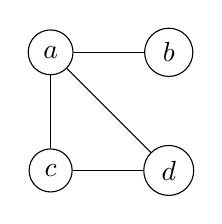
\begin{tikzpicture}[node distance={15mm}, main/.style ={draw, circle}]
    \node[main] (1) {$a$};
    \node[main] (2) [right of=1] {$b$};
    \node[main] (3) [below of=1] {$c$};
    \node[main] (4) [below of=2] {$d$};
    \draw (1) -- (2);
    \draw (1) -- (3);
    \draw (1) -- (4);
    \draw (3)--(4);
\end{tikzpicture}
\]
\[M = \{\{a,b\}, \{c,d\}\}\]
$M = \emptyset$ is a matching. 
\begin{definition}[Maximum Matching]
    A \emph{maximum matching} if it contains the greatest number of edges possible. 
\end{definition}
\noindent
\textbf{Example:}
\[
    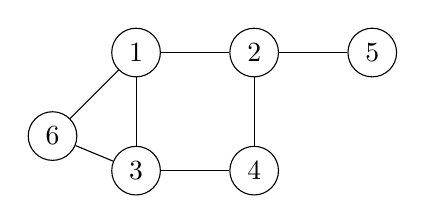
\begin{tikzpicture}[node distance={15mm}, main/.style ={draw, circle}]
        \node[main] (1) {1};
        \node[main] (2) [right of=1] {2};
        \node[main] (3) [below of=1] {3};
        \node[main] (4) [below of=2] {4};
        \node[main] (5) [right of=2] {5};
        \node[main] (6) [below left of=1] {6};
        \draw (1) -- (2);
        \draw (1) -- (3);
        \draw (3) -- (4);
        \draw (2)--(4);
        \draw (6)--(1);
        \draw (6)--(3);
        \draw (2) -- (5);
    \end{tikzpicture}
\]
\[M = \{\{6,3\}, \{6,1\}\}\]
This is not a maximum matching because we could add the edge $\{1,2\}$ to get a matching with 3 edges. So 
\[M = \{\{6,3\}, \{6,1\},\{2,1\} \}\]
This matching is maximum.
\begin{definition}[Perfect Matchings]
    A matching is \emph{perfect} if it matches \emph{all} vertices.
\end{definition}
\noindent
\textbf{Example:}
\[
    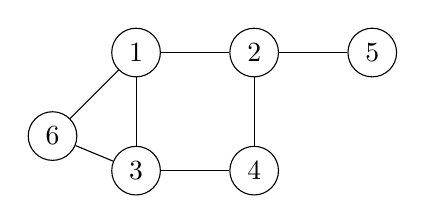
\begin{tikzpicture}[node distance={15mm}, main/.style ={draw, circle}]
        \node[main] (1) {1};
        \node[main] (2) [right of=1] {2};
        \node[main] (3) [below of=1] {3};
        \node[main] (4) [below of=2] {4};
        \node[main] (5) [right of=2] {5};
        \node[main] (6) [below left of=1] {6};
        \draw (1) -- (2);
        \draw (1) -- (3);
        \draw (3) -- (4);
        \draw (2)--(4);
        \draw (6)--(1);
        \draw (6)--(3);
        \draw (2) -- (5);
    \end{tikzpicture}
\]
\[M = \{\{6,3\}, \{6,1\},\{2,1\} \}\]
is a perfect matching. In general, if a graph has an odd number of vertices, it cannot have a perfect matching. 
\begin{theorem}
    Let $G = (V,E)$ be a graph whose set of edges is the union of two matchings. Then $G$ is bipartite. 
\end{theorem}
\begin{proof}
    Let $M_1$ and $M_2$ be the two matchings such that $E = M_1 \cup M_2$. We have to prove that $G$ does not have a cycle of odd length. By the previous theorem, this implies that $G$ is bipartite. For a contradiction, let 
    \[v_0, v_1, v_2, \ldots, v_{l-1}, v_0\]
    be a cycle of odd length. The edge $\{v_0, v_1\}$ is in $M_1$ or $M_2$. Without loss of generality, assume that $\{v_0, v_1\} \in M_1$. Then $\{v_1,v_2\} \in M_2$ otherwise $M_1$ would not be a matching. Then $\{v_2,v_3\} \in M_1$ and so on. So we have 
    \[\{v_i, v_{i+1}\} \in M_1 \text{ if $i$ is even}\]
    \[\{v_i, v_{i+1}\} \in M_2 \text{ if $i$ is odd}\]
    Then, $\{v_{l-2}, v_{l-1} \in M_2\}$ since $l -2$ is odd, and $\{v_{l-1}, v_0\} \in M_1$ since $l-1$ is even. But, the edge $\{v_0, v_1\}$ in $M_1$ shares an edge with $\{v_{l-1}, v_0\}$ in $M_1$. This is a contradiction since $M_1$ is a matching.
\end{proof}
\noindent
\textbf{Example:}
\[
    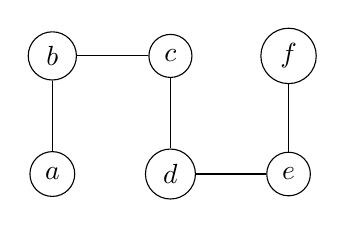
\begin{tikzpicture}[node distance={15mm}, main/.style ={draw, circle}]
        \node[main] (1) {$a$};
        \node[main] (2) [above of=1] {$b$};
        \node[main] (3) [right of=2] {$c$};
        \node[main] (4) [below of=3] {$d$};
        \node[main] (5) [right of=4] {$e$};
        \node[main] (6) [above of=5] {$f$};
        \draw (1) -- (2);
        \draw (2) -- (3);
        \draw (3) -- (4);
        \draw (4)--(5);
        \draw (5)--(6);
    \end{tikzpicture}
\]
\[M_1 = \{\{a,b\}, \{c,d\}, \{e,f\}\}\]
\[M_2 = \{\{b,c\}, \{d,e\}\}\]
$M_1 \cup M_2$ is equal to the set of edges. So this graph is bipartite. 

\chapter{More on Bipartite Graphs and Matchings}
\begin{definition}[Neighbour Set]
    Let $G = (V,E)$ be a graph. Let $S \subseteq V$. The \emph{neighbour set} of $S$, denoted $N(S)$ is the set of vertices having at least one neighbour in $S$. 
    \[N(S) = \{v \in V | \{v, s\} \text{ is an edge for some $s \in S$}\}\]
\end{definition}
\noindent
\textbf{Example:}
\[
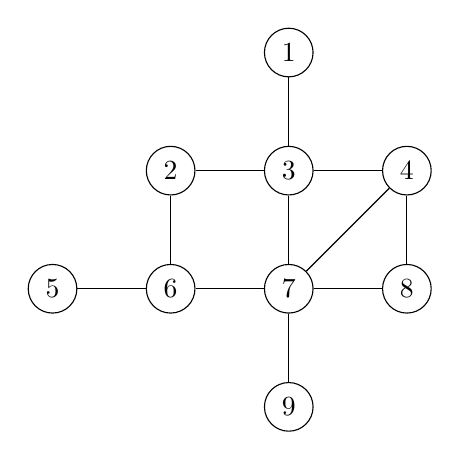
\begin{tikzpicture}[node distance={15mm}, main/.style ={draw, circle}]
    \node[main] (1) {1};
    \node[main] (2) [below of=1]{3};
    \node[main] (3) [left of=2]{2};
    \node[main] (4) [right of=2]{4};
    \node[main] (5) [below of=2]{7};
    \node[main] (6) [left of=5]{6};
    \node[main] (7) [right of=5]{8};
    \node[main] (8) [below of=5]{9};
    \node[main] (9) [left of=6] {5};
    \draw (1)--(2);
    \draw (2)--(3);
    \draw (2)--(4);
    \draw (2)--(5);
    \draw (5)--(6);
    \draw (5)--(7);
    \draw (5)--(8);
    \draw (6)--(9);
    \draw (4)--(5);
    \draw (4)--(7);
    \draw (3)--(6);
\end{tikzpicture}
\] 
\[N(\{3,4\}) = \{1,2,3,4,7,8\}\]
\[N(\{1\}) = \{3\}\]
\[N(\{2,3,4\}) = \{1,2,3,4,5,6,7,8,9\}\]
\begin{theorem}[Hall's Theorem]
    Let $G = (V,E)$ be a bipartite graph with partition $(A,B)$. There exists a matching that matches all vertices in $A$ if and only for every $S \subseteq A$. We have $|N(S)| \geq |S|$.
\end{theorem}
\begin{proof}
    ($\implies$) Suppose all vertices in $A$ can be matched. Let $S \subseteq A$ be a subset. We need to show that $|N(S)| \geq |S|$. For every $s \in S$, let $v$ be its partner in the matching. All these $v$'s are different. So there are $|S|$ of them. They are all neighbours of vertices in $S$. So they are in $N(S)$. Therefore, $|N(S)| \geq |S|$.\\[2ex]
    ($\impliedby$) Assume that for every subset $S \subseteq A$, we have $|N(S)| \geq |S|$. We want to prove that all vertices in $A$ can be matched. By indunction, 
    \begin{itemize}
        \item \textbf{Base Case: } $n = |A| = 1$. Then $|N(A)| \geq |A| = 1$. So the unique vertex in $A$ has a neighbour in $B$ and it can be matched.
        \item \textbf{Induction Hypothesis:} Let $K \geq 1$ be an integer. Assume that for all bipartite graphs $G$ with partition $(A,B)$ where $|A| \leq K$, if $|N(S)| \geq |S|$ for all $S \subseteq A$, then all vertices in $A$ can be matched.
        \item \textbf{Induction Step:} Let $G$ be a bipartite graph with partition $(A,B)$ where $|A| = k+1$. Consider two cases where for every $X \subset A$, we have $|N(X)| \geq |X| +1$, and there exists a subset $X \subset A$ such that 
        \[|N(X) < |X| +1 \implies |N(X)| = |X|\]
        \begin{itemize}
            \item \textbf{Case 1:} Let $a \in A$ and match it with an arbitrary neighbour $b \in B$. Remove $a$ and $b$ from $G$. Now for every proper subset $X \subset A$, we have $|N(X)| \geq |X|$. By the induction hypothesis, all vertices in $A \setminus \{a\}$ can be matched. So all vertices in $A$ can be matched.
            \item \textbf{Case 2:} Let $X \subset A$ be a proper subset such that $|N(X)| = |X|$. Observe that all subsets $X' \subseteq X$ are subsets of $A$, and $|N(X')| \geq |X'|$. So by the induction hypothesis, all vertices in $X$ can be matched. Remove all vertices in $X$ and $N(X)$ from $G$. Suppose we can show that for all subsets $Y \subseteq A \setminus X$, $Y$ has at least $|Y|$ neighbours in $B \setminus N(X)$, then we apply the induction hypothesis to match all vertices in $A \setminus X$. Combining the two matchings will give us a matching that matches all vertices in $A$. To prove our supposition, suppose for a contradiction that there exists a subset $Y \subseteq A \setminus X$ that has less than $|Y|$ neighbours in $B \setminus N(X)$. Then the vertices in $X \cup Y$ have less than $|N(X)| + |Y|$ neighbours in $G$. Then
            \begin{align*}
                |N(X \cup Y)| &< |N(X)| + |Y|\\
                &= |X| + |Y|\\
                &= |X \cup Y|\\
                &\leq |N(X \cup Y)|
            \end{align*}
            Which is a contradiction. 
        \end{itemize}
    \end{itemize}
\end{proof}
\end{document}

 